\documentclass[15pt,a4paper]{article}

%use the english line for english reports
%usepackage[english]{babel}
\usepackage[portuguese]{babel}
\usepackage[utf8]{inputenc}
\usepackage{indentfirst}
\usepackage{graphicx}
\usepackage{verbatim}
\usepackage{cite}
\usepackage{url}


\begin{document}

\setlength{\textwidth}{16cm}
\setlength{\textheight}{22cm}

\title{\Large\textbf{JogginGo!}\linebreak\linebreak\linebreak
\Large\textbf{Relatório Final}\linebreak\linebreak

\includegraphics[height=6cm, width=7cm]{feup.pdf}\linebreak \linebreak
\Large{Mestrado Integrado em Engenharia Informática e Computação} \linebreak \linebreak
\Large{Paradigmas de Programação}\linebreak
}

\author{ Luís Dias - 080509094 - ei08094@fe.up.pt \\ Luís Gomes - 080509169 - ei08169@fe.up.pt \\\linebreak\linebreak \\
\\ Faculdade de Engenharia da Universidade do Porto \\ Rua Roberto Frias, s\/n, 4200-465 Porto, Portugal \linebreak\linebreak\linebreak
\linebreak\linebreak\vspace{1cm}}
%\date{27 de Maio de 2013}
\maketitle
\thispagestyle{empty}

%************************************************************************************************
%************************************************************************************************

\newpage

\tableofcontents

%************************************************************************************************
%************************************************************************************************

%*************************************************************************************************
%************************************************************************************************

\newpage

\section{Resumo}

Com uma interface limpa e amiga do utilizador, o JogginGo! é uma aplicação Web que permite a gestão de todas as corridas feitas por qualquer utilizador registado. Cada corrida é um tratada como um conjunto de coordenadas GPS (\textit{Global Positioning System}) recolhidas com recurso aos sensores de um dispositivo móvel Android. A cada minuto, intervalo de tempo definido, é recolhida a posição em que o atleta se encontra, e o conjunto de pontos é assim representado visualmente na interface \textit{web}. 

\newpage
\section{Introdução}

Este projecto insere-se no âmbito da unidade curricular de Paradigmas de Programação, do 4º ano do Mestrado Integrado em Engenharia Informática e Computação da Faculdade de Engenharia da Universidade do Porto. Tendo em conta o conteúdo programático da unidade curricular, era esperado realizar um projecto que envolvesse mais do que um paradigma de programação e que as diferentes partes desenvolvidas interagissem entre si, de forma a criar um produto único e funcional.

\subsection{Objectivo}

O objectivo deste trabalho era criar uma plataforma \textit{mobile} de controlo de corridas de um determinado atleta. Do ponto de vista de utilização, foi necessário criar uma plataforma que permitisse a qualquer utilizador registar-se e visualizar todas suas corridas. Assim, desenvolvemos também um \textit{webservice} que preenchesse essa lacuna. Para além disso, é o \textit{webservice} o responsável por receber, tratar e armazenar os dados enviados pelo dispositivo móvel.

\subsection{Motivação}

A motivação principal deste projecto foi o desafio da integração de diferentes linguagens e paradigmas na criação de um produto único e funcional aplicado a um cenário real. 
Para além da componente académica, o desenvolvimento de um produto útil e enquadrado no mundo actual, com possibilidades de ser usado por qualquer atleta nas suas corridas, foi outra das motivações fulcrais. Achamos que o produto por nós desenvolvido responde às necessidades do público-alvo.


\newpage
\section{Descrição do Sistema Desenvolvido}

\subsection{Descrição Conceptual}

\subsubsection{Funcionalidades}

\textbf{Java (Android):}
\\

As tarefas disponibilizadas pela componente Java estão relacionadas com a aplicação Android. Esta é a responsável pela ligação com a parte funcionalmente mais importante do sistema, que é a captura de coordenadas durante a corrida de um utilizador. Assim que este termina a corrida e informa a aplicação que deseja sincronizar os dados, estes são enviados para a plataforma web.

\begin{itemize}
  \item \textit{GPSTracker:} Permite obter as coordenadas actuais do dispositivo móvel do utilizador. É, assim, responsável por comunicar estas alterações à aplicação, com um intervalo definido de 1 minuto, para que estas coordenadas possam ser guardadas para futura sincronização;

 \item \textit{DatabaseHandler} - Responsável por guardar as coordenadas obtidas e adicioná-las a uma pista, correspondente à corrida actual do utilizador. Estas são guardadas numa base de dados temporária  \textit{SQLite}, que guarda os dados da corrida até que o utilizador faz a sincronização com a plataforma ou decide descartá-la. 

 \item \textit{MapWithStats} - Depois de terminar a corrida, o utilizador poderá ver um mapa, recorrendo à  \textit{API }do \textit{Google Maps}, com o percurso efectuado. Poderá também ver um conjunto de estatísticas referentes à corrida, como velocidade média, distância percorrida e tempo total.

\end{itemize}
 
\textbf{Ruby on Rails:}
\\

A componente Ruby on Rails é a responsável pela plataforma  \textit{online} da aplicação. É, no fundo, a interface de comunicação com o utilizador, e é onde este se liga à vertente social da aplicação, onde pode competir de forma amigável pelos melhores tempos. 

\begin{itemize}

 \item \textit{Signup} - Permite ao utilizador registar-se na aplicação para poder usufruir das funcionalidades da aplicação.

 \item \textit{Login} - O utilizador entra na sua conta para poder ver os seus dados, corridas efectuadas e competir contra outros utilizadores.

 \item \textit{Logout} - Permite ao utilizador terminar a sessão actual.

 \item \textit{Test your limits} - Funcionalidade de competição amigável entre utilizadores, em que para determinado percurso o utilizador é desafiado a tentar obter o melhor tempo possível para ficar no  \textit{ranking} dos melhores tempos.

 \item \textit{MyStats} -  Permite que o utilizador veja os melhores tempos efectuados por ele, assim como distâncias mais longas e velocidades médias atingidas.

 \item \textit{AddTrack} -  Permite ao utilizador adicionar novas pistas para serem avaliadas como sendo passíveis de ser adicionadas às corridas do \textit{Test your Limits}, para que outros possam competir.

\end{itemize}


\subsubsection{Estrutura do Programa}

Este projecto ficou dividido em 2 módulos distintos: \textit{Webservice} e terminal Android. Relativamente ao \textit{Webservive}, e tal como referido ao longo deste documento, é o responsável pela autenticação do utilizador, assim como pelo tratamento de toda a informação recebida do dispositivo móvel. Após receber a informação, o \textit{webservice} analiza-a e guarda-a na base de dados, para mais tarde proceder à sua representação recorrendo a API do Google Maps. De notar que o dispositivo móvel apenas transmite ao \textit{webservice} os percursos que ainda não tenham sido sincronizados.


\begin{figure}[htp]
  \centering
  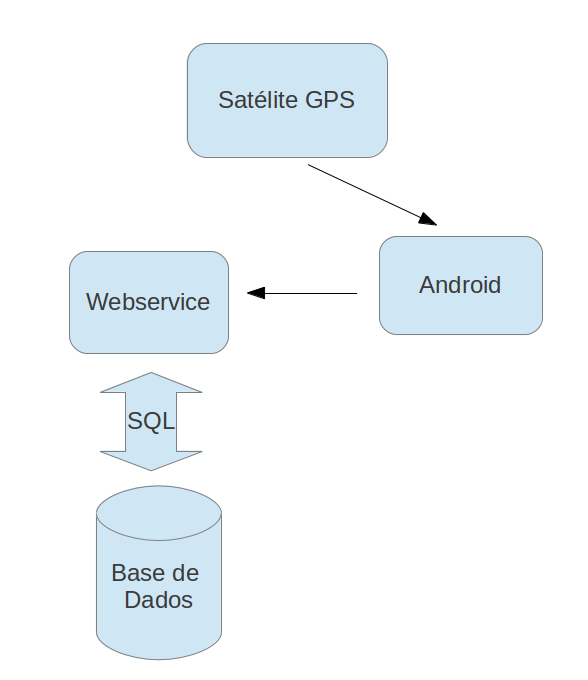
\includegraphics[scale=0.5]{diagrama.png}
  \caption{Estrutura do programa}
\end{figure}

O segundo módulo, ou seja, o terminal Android, trata da recolha das coordenadas GPS e do seu correcto armazenamento, numa base de dados SQLite, até que seja feita a sincronização com o \textit{Webservice}. Para além da recolha, é também da sua responsabilidade a criação de um documento JSON utilizado como base para a comunicação com o terminal web.


\subsubsection{Linguagens de Programação }


\textbf{Java:}

Para o JogginGo! foi utilizada a linguagem Java para o desenvolvimento da aplicação Android, utilizando o SDK existente para o efeito. É responsável, assim, pela obtenção de coordenada GPS do dispositivo móvel, pela criação de uma base de dados relacional SQLite e pela comunicação REST com o \textit{webservice}. 

A linguagem Java é multi-paradigma, e para este projecto foi utilizada principamente como linguagem mobile e orientada a objectos. O principal factor para a escolha do Java foi o seu excelente comportamento na programação Android, assim como a facilidade de criação de uma base de dados SQLite utilizando objectos. Para além disto, contou muito a familiarização com a linguagem, o que permitiu maior agilidade de desenvolvimento e menos tempo perdido na resolução de problemas.
\\

\textbf{Ruby:}
\\

Para o desenvolvimento do webservice da aplicação, que ao mesmo tempo é a plataforma online, foi utilizado Ruby, principalmente devido à framework Ruby on Rails que permite prototipagem rápida e eficiente. Esta framework tem uma estrutura MVC (Model-View-Controller) que permite facilmente separar a lógica do servidor (back-end) da interface com o utilizador (Front-End). Foi assim utilizada para todo o desenvolvimento de todas as funcionalidades da plataforma online e para criação da base de dados. 

A linguagem Ruby também é multi-paradigma, e aqui foram usadas várias vertentes da mesma (orientada a objetos, scripting e reflexiva), tanto através da utilização de classes, do embeber de partes do código dentro de HTML ou Javascript e da utilização e carregamento de plugins (com novas classes) em tempo de execução . Para o desenvolvimento da plataforma foi equacionada a utilização de Python com a framework Django, mas depois de alguma pesquisa foi seleccionado o Ruby (on Rails) devido à facilidade com que se manipula a base de dados, à existência de inúmeros \textit{plugins} que nos podem ajudar a melhorar a plataforma e também porque o Django é mais indicado para uma prototipagem rápida de ferramentas de administração, e menos de componentes com muitos utilizadores (como redes sociais) e muitas funcionalidades distintas.
\\

\textbf{Javascript:}
\\

Foi utilizado Javascript principalmente para uma melhor interacção do utilizador com a plataforma. A sua escolha deveu-se a ser, até ao momento, a única linguagem que permite a realização das suas funcionalidades na web e porque possui a biblioca JQuery que é também a mais utilizada na framework (Ruby on Rails) utilizada para o desenvolvimento da plataforma, que permite alterações ao Domain Objec Model (DOM) das páginas em tempo-real, sem necessidade de fazer novos pedidos ao servidor. Apesar de ser multi-paradigma, foi utilizada como linguagem de \textit{scripting}, já que permite que o seu código esteja embebido noutras linguagens e não requerer qualquer tipo de compilação, sendo o seu código totalmente \textit{client-side}, ou seja, executado na máquina do utilizador.

\section{Implementação}

\subsection{Ambiente de desenvolvimento}

Para os diferentes módulos, foram usadas diferentes tecnologias e ambientes.

O \textit{Webservice} foi desenvolvido em utilizando a tecnologia Ruby on Rails, com a ajuda da API do Google Maps, programado no editor de texto Sublime Text, recorrendo a um servidor local (localhost). Mais tarde, fizemos a migração da plataforma para o sistema de cloud, Heroku.

Relativamente ao terminal móvel, foi desenvolvida em Java (Android), recorrendo ao IDE Eclipse. 

Ambos os modelos foram desenvolvidos em computadores portáteis utilizando o sistema operativo Linux (Ubuntu).


\newpage
\section{Conclusão}

As conclusões deste projecto são positivas em vários níveis. O facto de utilizarmos diferentes linguagens de programação e paradigmas para o desenvolvimento de um projecto torna-se um desafio e a maior motivação de desenvolvimento. 

O facto de ser uma aplicação com um factor de utilidade real bastante elevado fez com que a satisfação pessoal fosse outro dos factores de grande motivação.

Foi também um bom desafio o desenvolvimento da aplicação Android que fosse capaz de recolher as coordenadas \textit{GPS} ao longo duma corrida, já que não era algo que nenhum dos elementos tivesse experimentado. Para além disso, conseguir ligar estas coordenadas e a um mapa e ao mesmo tempo extrair informações tal como velocidade média, tempo e distâncias percorridas tornou-se bastante positivo.

Para desenvolvimento futuro, seria interessante o desenvolvimento de algumas funcionalidades que desejávamos ter implementado e que permitissem algum destaque face às diferentes aplicações semelhantes existentes no mercado, e ao mesmo tempo adicionar mais funcionalidades da plataforma \textit{online} à aplicação Android e melhorar a sua usabilidade e potencial.


\section{Melhoramentos}

Há alguns melhoramentos que tínhamos em vista, no caso de ter existido mais tempo para a sua implementação. Dos mais importante, destacaríamos o melhoramento da interface gráfica, que neste momento se encontra pouco cuidada pois decidimos dar mais ênfase às funcionalidades do que à usabilidade.

Outro dos melhoramentos que achamos que traría mais valor ao nosso projecto, era a inclusão da funcionalidade “Test your Limits”, que permitiria a um qualquer atleta registado, competir num percurso pré-definido pela plataforma.

\section{Bibliografia}

\subsection{Publicações}

\subsection{URLs}

\begin{itemize}
\item Storage Options, \emph{http://developer.android.com/guide/topics/data/data-storage.html
}, Maio 2013
\item Google Developers, \emph{https://developers.google.com/maps/}, Maio 2013

\item Latitude and Longitude of a Point, \emph{http://itouchmap.com/latlong.html}, Maio 2013
\item GMaps4Rails, \emph{https://github.com/apneadiving/Google-Maps-for-Rails}, Maio 2013

\item Stack Overflow, \emph{http://stackoverflow.com}, Maio 2013

\item Android GPS, \emph{http://www.androidhive.info/2012/07/android-gps-location-manager-tutorial/}, Maio 2013

\item Google Maps Android API V2, \emph{https://developers.google.com/maps/documentation/android/start\_the\_google\_maps\_api\_key}, Maio 2013

\end{itemize}



\newpage
\appendix
\section{Apêndice}
\subsection{Manual de Utilização}


\end{document}